\subsubsection{Pregled plata zaposlenih}
\label{subsubsec:vozni park}
\begin{itemize}
  \item \textbf{Kratak opis}: Računovođa može da zatraži pregled plata zaposlenih u određenom vremenskom trenutku. Kada dobije željeni izveštaj, 
  može ga sačuvati na sistemu, izmeniti ili odštampati.

  \item \textbf{Učesnici}:
    \begin{itemize}
    \item Računovođa.
    \end{itemize}
  \item \textbf{Preduslovi}:
    \begin{itemize}
    \item  Računovođa je uspešno ulogovan na sistem auto škole.
    \item  Sistem je dostupan.
    \item  Računovođa ima pristup internetu.
    \end{itemize}
  \item \textbf{Postuslovi}:
      \begin{itemize}
      \item  Računovođa je dobio izveštaj o zahtevanim platama za zaposlene.
      \item  Računovođa je uspešno izvršio željene izmene plata.
      \end{itemize}
  \item \textbf{Osnovni tok}:
      \begin{enumerate}
        \item Računovođa otvara stranicu za uvid u spisak zaposlenih radnika i njihovih plata u željenom periodu.
        \item Sistem prikazuje trenutno zaposlene kao i njihove plate.
        \item Računovođa bira dugme "Izmeni" da promeni platu ili  "Odštampaj" za dobijanje izveštaja.
        \item Sistem omogućava računovođi da izmeni podatke u tabeli  ili  izvrši štampanje.
        \item Računovođa potvrđuje izmene ili vrši štampanje.
        \item Sistem evidentira izmene.
      \end{enumerate}

  \item \textbf{Alternativni tokovi}:
      \begin{itemize}
        \item A1. \textbf{Ne mogu se dobiti traženi podaci.}
        Ako sistem u koraku 2 ne može iz nekog razloga da prikaže tražene podatke, računovođa se obaveštava da je došlo do problema.
        Proces se nastavlja od koraka 1 osnovnog toka.
        \item A1. \textbf{Neuspela izmena ili štampanje.}
        Ako u koraku 5 štampač nije dostupan ili su uneti podaci nevalidni, računovođa se obaveštava o problemu. Proces se nastavlja unošenjem
        validnih podataka u slučaju izmene i nastavlja se od koraka 4. U slučaju nedostupnosti štampača proces se završava.
      \end{itemize}

      
  \item \textbf{Dodatne informacije}:
      \begin{itemize}
        \item Podaci o zaposlenom : ime, prezime, jmbg, broj telefona, plata.
      \end{itemize}
\end{itemize}

\begin{figure}[H]
  \begin{center}
      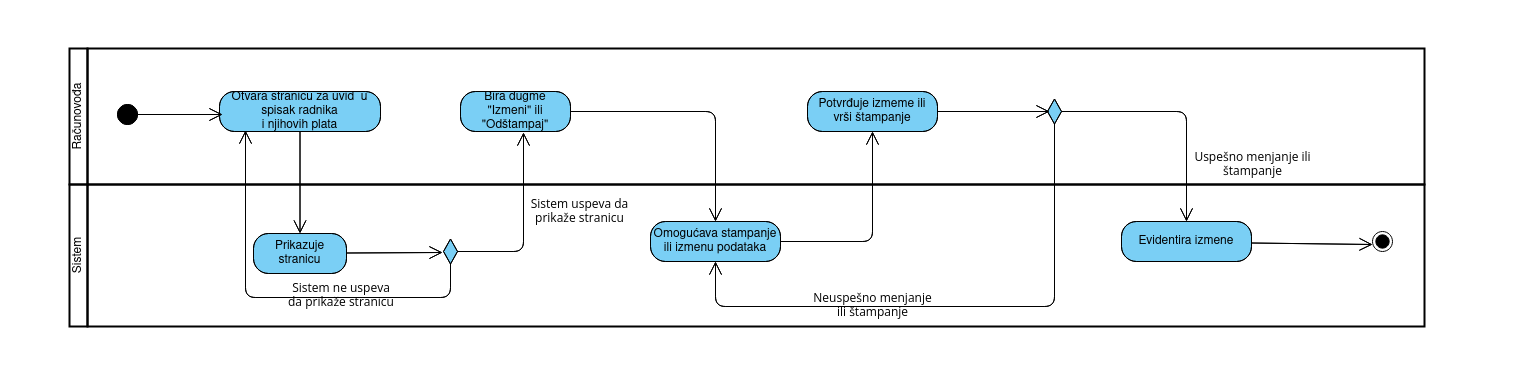
\includegraphics[width=140mm, height=70mm]{Diagrams/pregled_zaposlenih.png}
  \end{center}
  \caption {Dijagram aktivnosti - Pregled plata zaposlenih}
  \label{activity_pregled_zaposlenih}

\end{figure}
